\section{Geomagic touch}\label{sec:geo_magic}
The Geomagic Touch(GT) is a haptic feedback controller device, %\textcolor{red}{which has the ability to manipulate its joints in such a way that the user feels resistance when moving the pin in a certain direction or way.}
that is able to output force to the user, and arbitrarily resist the user's attempts at moving the controller.
	 The Geomagic Touch described in this section can be seen on \figref{fig:phantom_omni}.

\begin{figure}[H]
	\centering
	\begin{subfigure}{.45\textwidth}
		\centering
		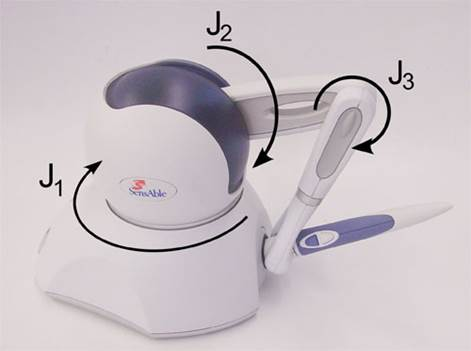
\includegraphics[width=\linewidth]{haptick1.png}
		\caption{Overview of the Geomagic Touch's first three joints.}
		\label{fig:phantom1}
	\end{subfigure}
	\begin{subfigure}{.45\textwidth}
		\centering
		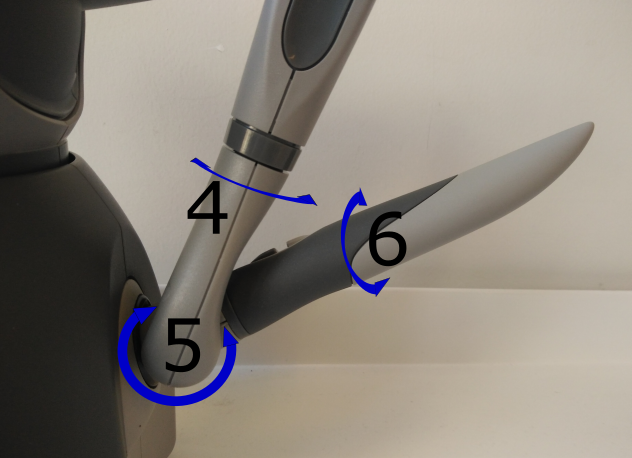
\includegraphics[width=\linewidth,height=5.4cm]{haptick2.png}
		\caption{Overview of the Geomagic Touch's last three joints}
		\label{fig:phantom2}
	\end{subfigure}
\caption{Overview of all the Geomagic Touch's joints.}
\label{fig:phantom_omni}
\end{figure}

 On \figref{fig:phantom_omni}, it can be seen that the Geomagic Touch has six \gls{DOF}, where only the first three can be actuated, see \figref{fig:phantom1}. This means that the device only has the ability to generate translational force feedback with three \gls{DOF}.% in this case roll, pitch and yaw.

The GT communicates with the computer through User Datagram Protocol (UDP). This communication can be established directly through an ethernet cable or by plugging the ethernet cable into USB converter. The interfacing is shown on \figref{interface}. The Geomagic Touch was programmed and the connection was established using a C++ based application programming interface (API). The API provides force rendering,  virtual environment and position measurement features. The present project utilizes force rendering capabilities to provide force feedback and measures the GT's position as an input to the system.